\chapter{Introdução}
\label{cap:introducao}
Considerado com ponto-chave para a Web Semântica \cite{berners2001semantic}, o conceito de Dados Conectados vem sendo abordado de forma crescente por acadêmicos, governos e empresas. Tal crescimento se deve ao fato de Dados Conectados ser alternativa relevante para conectar bases de dados distribuídas na Web. Segundo \citeonline{hyland2011joy}, Dados Conectados se trata de um conjunto de boas práticas para publicar e conectar dados estruturados na Web. Ademais, \citeonline{berners2006linked} afirma que Dados Conectados não é apenas por dados na internet, mas fazer conexões entre eles, permitindo assim, que pessoas ou máquinas possam explorar a Web dos dados.

Web de Dados bem como Web dos Documentos, são termos utilizados para descrever o paradigma da Web atualmente, onde o primeiro, que tem como base o segundo, reflete a possibilidade de conectar os dados através de links. Sendo esta, uma possibilidade inexistente quando se fala de Web dos Documentos, pois nesta, os documentos apontam para outros documentos através de links. 

O conceito Dados Conectados pode ser visto sob as perspectivas de consumo e publicação. A primeira aborda o ponto de vista do consumidor de Dados Conectados, tratando a exploração de dados para tornar as aplicações mais ricas. A segunda está sob a perspectiva do publicador, abordando processos \cite{bizer2007publish, hyland2011joy, villazon2011methodological, Avila2015} e conceitos \cite{berners2006linked, wood2014linked} necessários para publicar e manter os dados na Web de forma conectada. O processo de publicação de dados conectados envolve diferentes etapas, ferramentas e boas práticas \cite{world2014best} para a esperada qualidade dos dados publicados. 

A necessidade de levar em consideração tantos elementos fazem com que publicar dados conectados se torne não trivial. Um bom exemplo de tal complexidade é o modelo de processos proposto por \citeonline{Avila2015}, que pode ser visto na Figura \ref{fig:modelo_processo} , possuindo dezenas de tarefas ao longo do processo de publicação. Além disso, o mesmo contém etapas como reuso de vocabulários, conversão  e enriquecimento de dados, sendo esta última responsável por conectar os dados entre bases de dados distintas, que de acordo com \citeonline{berners2006linked} é impressindível para a existência de dados conectados.

\begin{figure}[!ht]
	\centering
	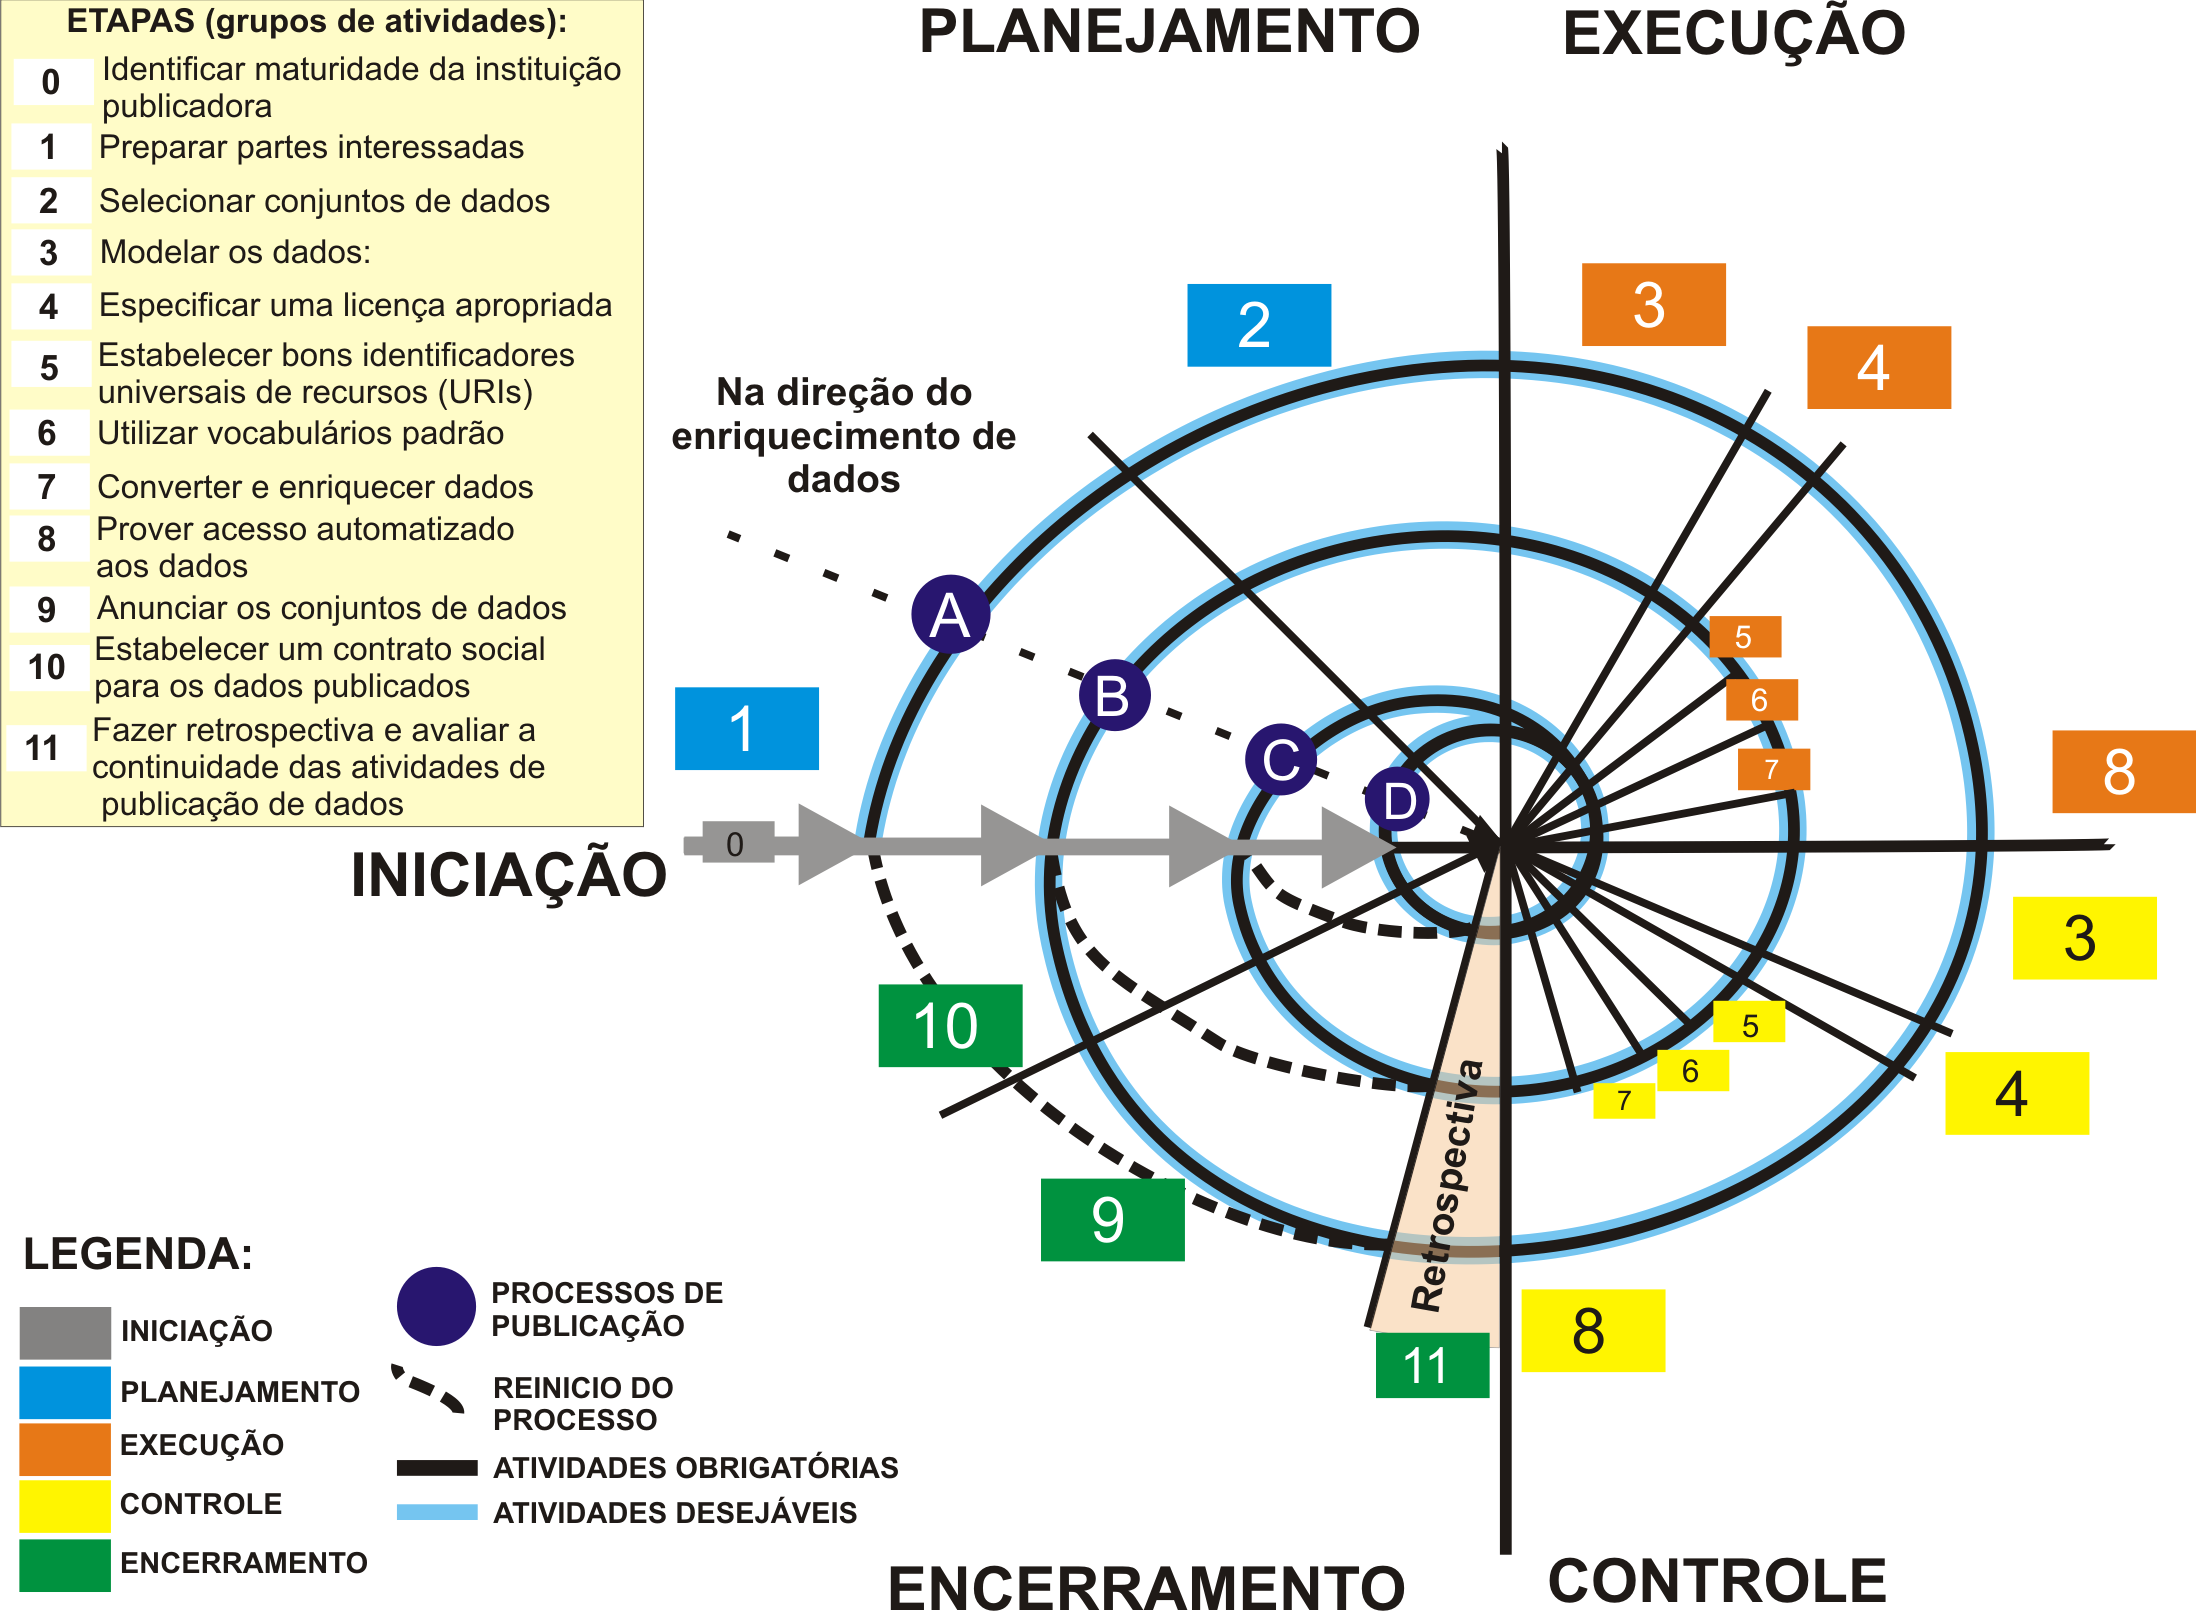
\includegraphics[width=0.95\textwidth]{./imagens/modelo-de-processo.png}\\
    \caption{Modelo de processo para a publicação de dados conectados governamentais}
	\footnotesize{Fonte: \cite{Avila2015}.}
	\label{fig:modelo_processo}
\end{figure}

Para o estabelecimento da relação semântica entre dados, utiliza-se ontologias e vocabulários, que podem ser entendidos como artefatos computacionais utilizados para a representação de um determinado universo de discurso. Dessa forma, o uso de ontologias está fortemente relacionado à interoperabilidade de dados \cite{guarino1998formal, simon2004using, farinelli2013papel}. Segundo o IEEE\footnote{\url{https://www.ieee.org/education_careers/education/standards/standards_glossary.html}}, interoperabilidade pode ser entendida como a capacidade de um sistema conversar de forma transparente com outro, sendo assim, interoperabilidade de dados pode ser entendido como a capacidade de um sistema de processar os dados de outro com esforço mínimo. 

Apesar da facilidade fornecida pelas ontologias em interoperar dados, criar conexão entre conjuntos de dados distintos mantem-se uma tarefa complexa, pois requer uma análise preliminar e detalhada por parte do especialista de domínio. Além disso, 
A conexão entre diferentes conjuntos de dados pode ser feita no nível conceitual, através do alinhamento de ontologias e no nível de dados, através do alinhamento de instâncias.

%Sendo necessário também aplicar técnicas de alinhamento entre os conjuntos de dados \cite{Castano2008}. Este problema também é reconhecido pelas comunidades de bancos de dados e integração de dados através do termo inglês record linkage \cite{gu2003record}, que se refere à tarefa de identificar com acurácia e de forma rápida registros correspondentes para a mesma entidade a partir de uma ou mais fontes de dados.

%Conhecido também como Problema de Resolução de Entidades \cite{menestrina2005generic} (do inglês Entity Resolution Problem) e deduplicação \cite{sarawagi2002interactive} (do inglês Deduplication), tratando-se de um processo que tem como objetivo identificar e mesclar recursos julgados representar a mesma entidade do mundo real. Além disso, é possível ressaltar outras áreas que podem se beneficiar a partir da conexão entre dados, sendo elas: 
%\begin{itemize}
%    \item \textbf{Integração semântica de dados}: Refere-se ao melhoramento de as técnicas existentes pra descobertas de mapeamento (semi) automático entre ontologias heterogêneas e distribuídas; 

%    \item \textbf{Reconhecimento de identidade}: Refere-se à capacidade de identificar se descritores de recursos distintos estão relacionados à mesma entidade do mundo real; 

%    \item \textbf{População de ontologias}: Refere-se a descoberta de relacionamentos entre novas instâncias e as instâncias já existentes na base de conhecimento. 
%\end{itemize}

%Por exemplo, admitindo a existência de uma entidade do mundo real (e.g. Pesquisador) onde atributos como nome e endereço estão armazenados em datasets distintos, onde estão vinculados a recursos que usam as seguintes URIs (http://www.ic.ufal.br/dac/rbie/author/615 e http://lattes.cnpq.br/4038730280834132) como na Figura \ref{fig:modelo_semantico}. Neste cenário, não é possível determinar, apenas através do alinhamento entre as ontologias, que ambas URIs fazem referência a mesma entidade, sendo necessário analisar informações adicionais provenientes de conexões semânticas entre conceitos e relações presentes nestes dados [31, 35]. 

%\begin{figure}[!ht]
%	\centering
%	\includegraphics[width=0.95\textwidth]{./imagens/researcher.png}\\
%    \caption{Relação entre entidade do mundo real, dados e modelo semântico}
%	\footnotesize{Fonte: Próprio autor.}
%	\label{fig:modelo_semantico}
%\end{figure}
%No cenário de publicação de Dados Conectados, criar conexões entre conjuntos de dados é uma tarefa custosa, pois requer análise preliminar e detalhada por um especialista de domínio. 

%Além disso, com a crescente quantidade de dados que estão sendo publicados Web, conforme a Figura \ref{fig:oferta_2020}, conectar esses dados se torna cada vez mais desafiador. Por exemplo, o catálogo de dados do governo de São Paulo2, que até o presente momento contém 424 conjuntos de dados, possui apenas 13 (0.23\%) que disponibiliza seus dados através de alguma serialização RDF (Turtle, RDF/XML).  


%AQUI, PRECISA ESCREVER SOBRE TÉCNICAS APLICADAS POR OUTROS TRABALHOS (RELACIONADOS) E DIZER POR QUE ELES NÃO RESOLVEM O PROBLEMA.  

%DEPOIS DISSO, DIZER QUE UM CAMINHO DE SOLUÇÃO É O ALINHAMENTO USANDO XXXXXXXXX E/OU YYYYYYYYYYY.  

%Dessa forma, pretende-se dispor uma abordagem semi-automática para publicar Dados Conectados, a partir de dados estruturados (publicado e não publicados na Web), levando em consideração, técnicas de alinhamento de dados, contribuindo assim, para o cenário de publicação de Dados Conectados. 

%Figura 2 - Oferta de dados na Web até 2020. Fonte: EMC 2012 
%\begin{figure}[!ht]
%	\centering
%	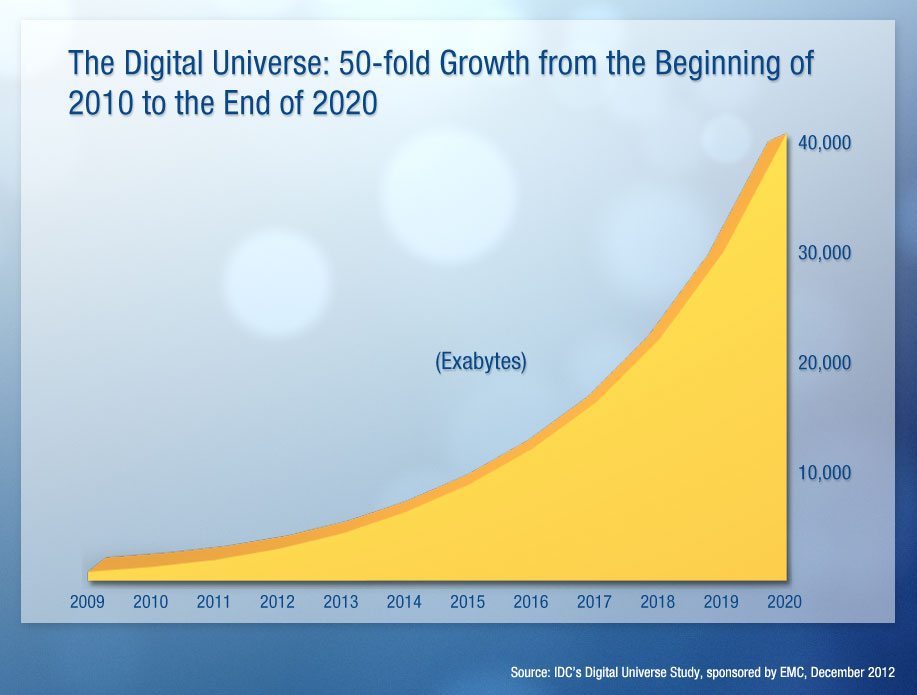
\includegraphics[width=0.8\textwidth]{./imagens/oferta.png}\\
%    \caption{Oferta de dados na Web até 2020}
%	\footnotesize{Fonte: EMC 2012.}
%	\label{fig:oferta_2020}
%\end{figure}



\subsection*{Contextualização}

\subsection*{Problemática}

\subsection*{Solucionática}

\subsection*{Objetivos}

\subsubsection*{Objetivo Geral}

\begin{itemize}
	\item Objetivo geral.
\end{itemize}

\subsubsection*{Objetivos específicos}
\begin{itemize}
\item Objetivo específico 1;
\item Objetivo específico 2;
\item Objetivo específico 3;
\item Objetivo específico 4.
\end{itemize}

\subsection*{Estrutura do trabalho}

O restante do trabalho está estruturado como segue:

\begin{enumerate}
\item[a)] \textbf{Seção 2} - descrição;
\item[b)] \textbf{Seção 3} - descrição;
\item[c)] \textbf{Seção 4} - descrição;
\item[d)] \textbf{Seção 5} - descrição;
\item[e)] \textbf{Seção 6} - descrição;
\item[f)] \textbf{Seção 7} - descrição;
\end{enumerate}
